\hypertarget{main_8c}{
\section{Referencia del Archivo main.c}
\label{main_8c}\index{main.c@{main.c}}
}


\subsection{Descripci\'{o}n detallada}
Programa principal, usa y prueba la libreria genesting. 

Definici\'{o}n en el archivo \hyperlink{main_8c-source}{main.c}.

{\tt \#include $<$stdio.h$>$}\par
{\tt \#include $<$stdlib.h$>$}\par
{\tt \#include $<$math.h$>$}\par
{\tt \#include \char`\"{}genesting.h\char`\"{}}\par
{\tt \#include \char`\"{}graphics.h\char`\"{}}\par
{\tt \#include \char`\"{}distance.h\char`\"{}}\par
{\tt \#include \char`\"{}population.h\char`\"{}}\par


Dependencia gr\'{a}fica adjunta para main.c:\begin{figure}[H]
\begin{center}
\leavevmode
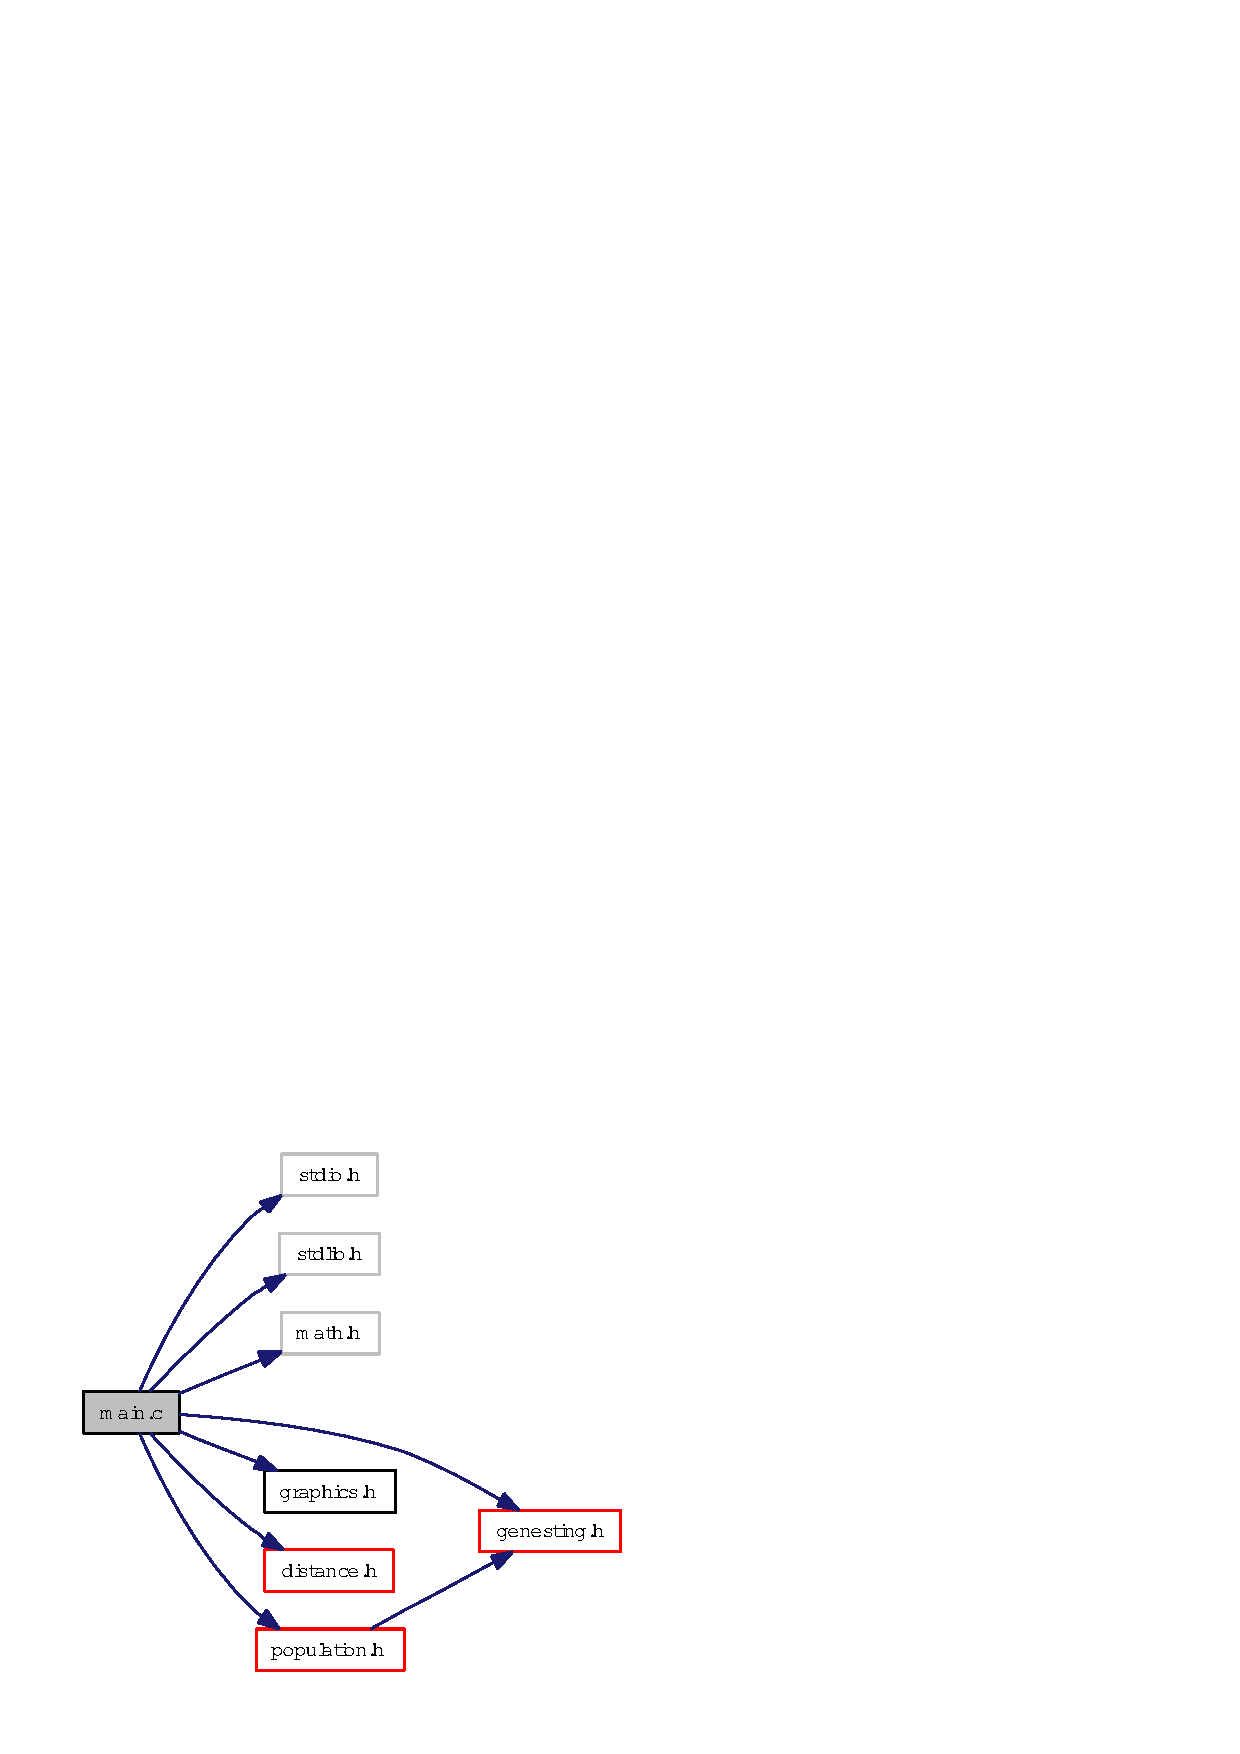
\includegraphics[width=151pt]{main_8c__incl}
\end{center}
\end{figure}
\subsection*{Funciones}
\begin{CompactItemize}
\item 
int \hyperlink{main_8c_3c04138a5bfe5d72780bb7e82a18e627_3c04138a5bfe5d72780bb7e82a18e627}{main} (int argc, char $\ast$$\ast$argv)
\end{CompactItemize}


\subsection{Documentaci\'{o}n de las funciones}
\hypertarget{main_8c_3c04138a5bfe5d72780bb7e82a18e627_3c04138a5bfe5d72780bb7e82a18e627}{
\index{main.c@{main.c}!main@{main}}
\index{main@{main}!main.c@{main.c}}
\subsubsection[main]{\setlength{\rightskip}{0pt plus 5cm}int main (int {\em argc}, char $\ast$$\ast$ {\em argv})}}
\label{main_8c_3c04138a5bfe5d72780bb7e82a18e627_3c04138a5bfe5d72780bb7e82a18e627}




Definici\'{o}n en la l\'{\i}nea 82 del archivo main.c.

\begin{Code}\begin{verbatim}83 {
84     genesting *g;
85     population *p;
86 
87 #if graphics
88 
89     init_graphics();
90 #endif
91 
92     if (argc<2)
93     {
94         fprintf(stderr,"Se deben entrar ingresar el nombre del archivo a leer\n");
95         return 1;
96     }
97 
98     g=leer_archivo(argv[1]);
99     p=(population*) malloc(sizeof(population));
100 
101     srand((int)p);
102 
103     genesting_init(g);
104 
105     genesting_show(g);
106 
107     population_create(p,g, 200);
108 
109     int i,k;
110     for (k=0;k<30;k++)
111     {
112         printf("Iteracion: %i\n",k);
113 
114         /*
115         for (i=0;i<5;i++)
116         {
117             printf("Individuo %i: [%i] \n",i,p->individuos[i].ngenes);
118             for (j=0;j<p->individuos[i].ngenes;j++)
119             {
120                 printf("Pat[%i] x[%f] y[%f] t[%f]\n",
121                        p->individuos[i].posgen[j].id,
122                        p->individuos[i].posgen[j].x,
123                        p->individuos[i].posgen[j].y,
124                        p->individuos[i].posgen[j].t);
125             }
126         }
127         */
128         population_evaluate(p);
129 
130         for (i=0;i<10;i++)
131         {
132             printf("Individuo %i: [%i] fitness: %f areautil: %f\n",i,p->individuos[i].ngenes,p->individuos[i].fitness,p->individuos[i].areautil);
133             /*
134                         for (j=0;j<p->individuos[i].ngenes;j++)
135                         {
136                             printf("Pat[%i] x[%f] y[%f] t[%f]\n",
137                                    p->individuos[i].posgen[j].id,
138                                    p->individuos[i].posgen[j].x,
139                                    p->individuos[i].posgen[j].y,
140                                    p->individuos[i].posgen[j].t);
141                         }
142             */
143         }
144 
145         population_generation(p);
146     }
147     free(p);
148 
149     return 0;
150 }
\end{verbatim}\end{Code}




Gr\'{a}fico de llamadas para esta funci\'{o}n:\begin{figure}[H]
\begin{center}
\leavevmode
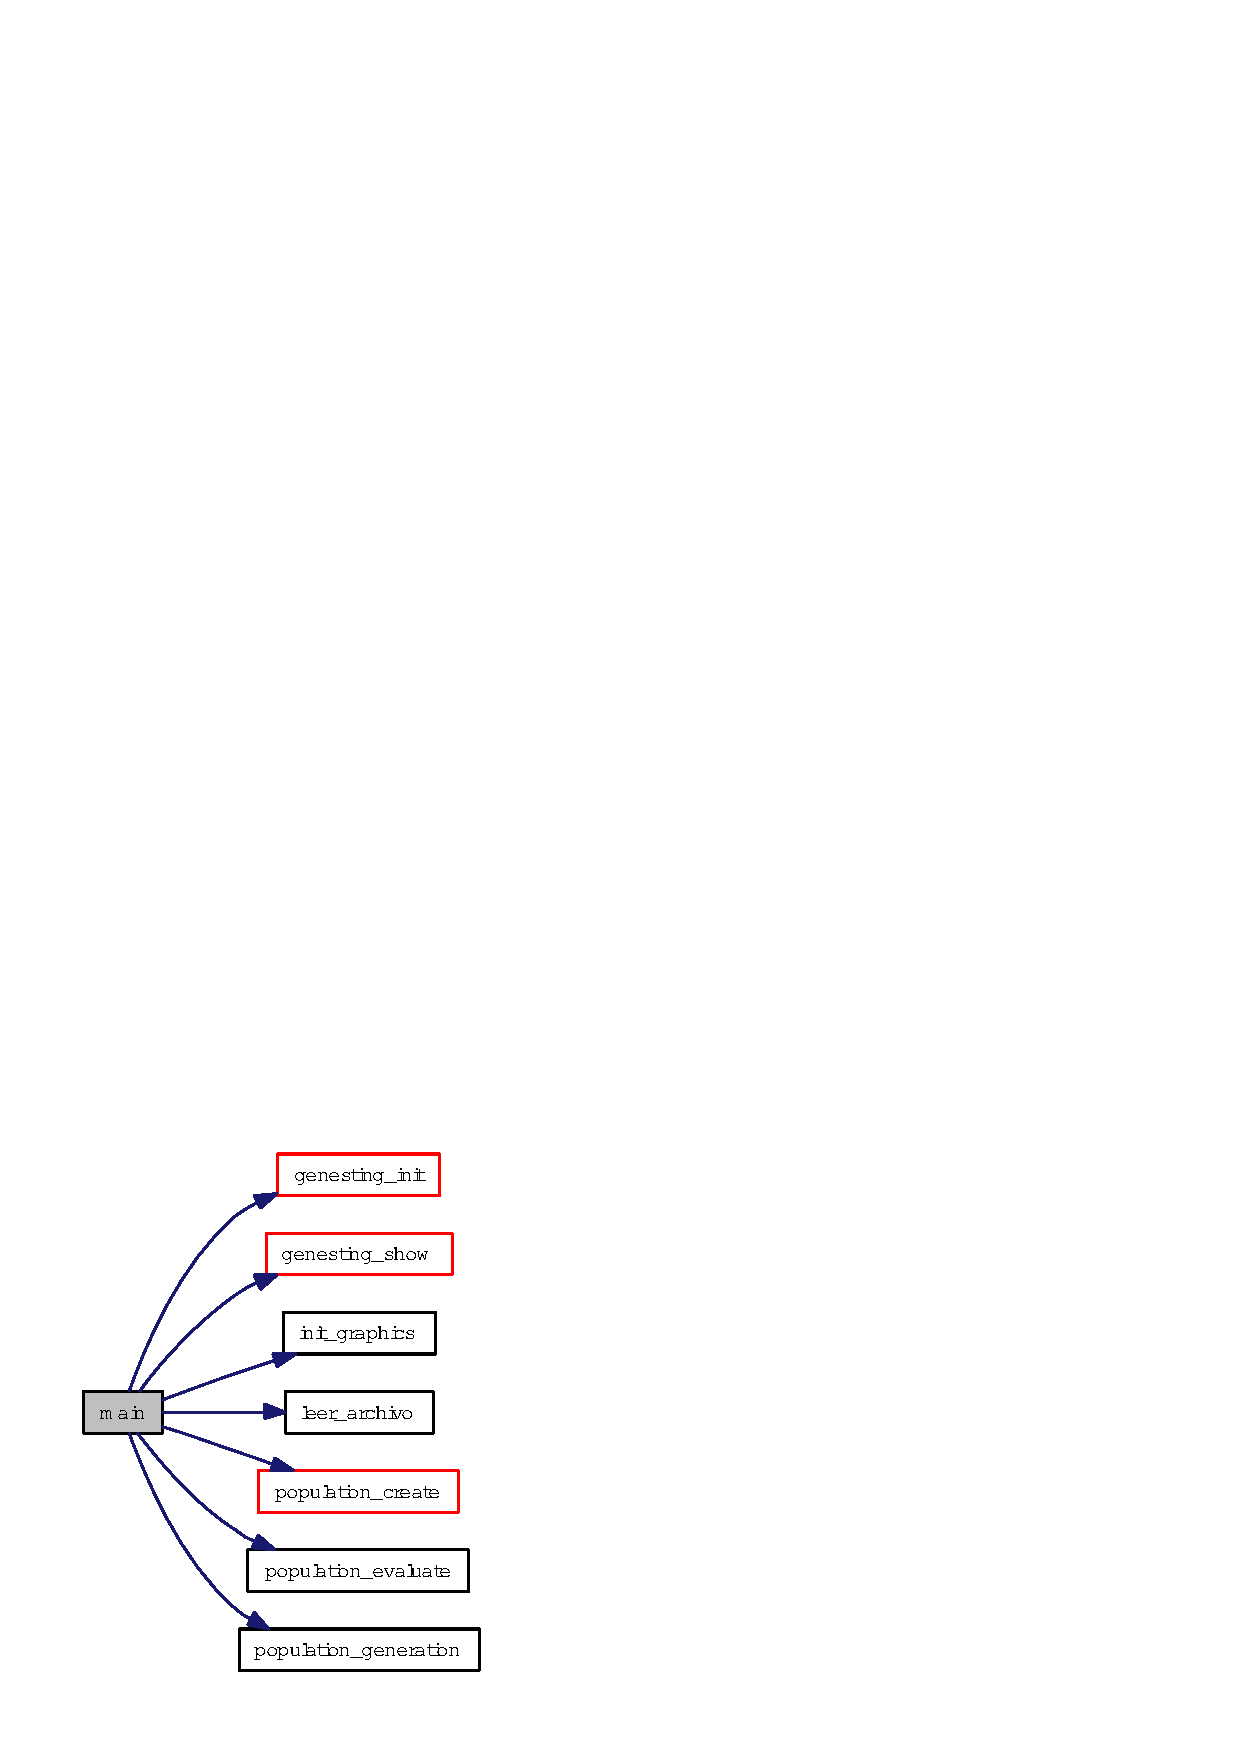
\includegraphics[width=117pt]{main_8c_3c04138a5bfe5d72780bb7e82a18e627_3c04138a5bfe5d72780bb7e82a18e627_cgraph}
\end{center}
\end{figure}
